% !TeX spellcheck = en_GB
\section{Theoretical Background}
In the following some physical concepts needed for the understanding of this experiment are explained.
%\subsection{Physical Concepts}
\subsection{Colour Centres}

Diamond structure is well known and studied in crystallography, its lattice consist of a cubic structure of eight carbon atoms. Basically consists of two face-centred cubic lattices, where the face centred atoms of one cell build the vertices of the other \cite{sir_c_v_raman_crystal_1944}. Since there are only  identical atoms per unit cell, there is no absorption of photon in the IR-region \cite{mildren_1_nodate}, This mean that a pure diamond can not have fluorescence properties (in first order) but this properties can be achieved by changes due to impurities in the structure. Such impurities are called colour centres.

These Colour centres (CC) are a kind of defect in crystal structures which contain a electron that absorbs light of certain wavelengths \cite{lesik_engineering_2015}. This basic defect in the regular spacing of atoms, absorbs visible light of a particular colour, lending a characteristic colour to the solid. \\

There are more then 100 luminescent defects in diamond \cite{jelezko_single_2006}. Colour centres results from the absence of a negatively charged ion from a particular point in an ionic solid. This vacancy which acts like a positively charged particle attracts and traps an electron, and their combination constitutes an Colour-centre \cite{choudhury_principles_2014}. One of the most abundant and also studied one is the Nitrogen-Vacancy centre, because  nitrogen is a prominent impurity in the material. In the next section we will talk in more detail about its properties.


\subsection{NV-Centres in Diamonds}
\label{sec:nvcentres}
 The NV-centres are a defect or impurities in the diamond structure, where two carbon atoms are missing, one of them being filled by a Nitrogen atom, the other position staying vacant. NV-centres occur in a diamond in four different configurations. In figure \ref{fig:nclatt} there is shown the basic diamond lattice including the four possible configurations of the NV-centre. NV-centres can exist in two charge states, the neutral NV$^{0}$ state and the negatively charged NV$^{-}$ state that have different energy levels and allowed transitions \cite{pham_magnetic_nodate}.\\
 
 \begin{figure}
 	\centering
 	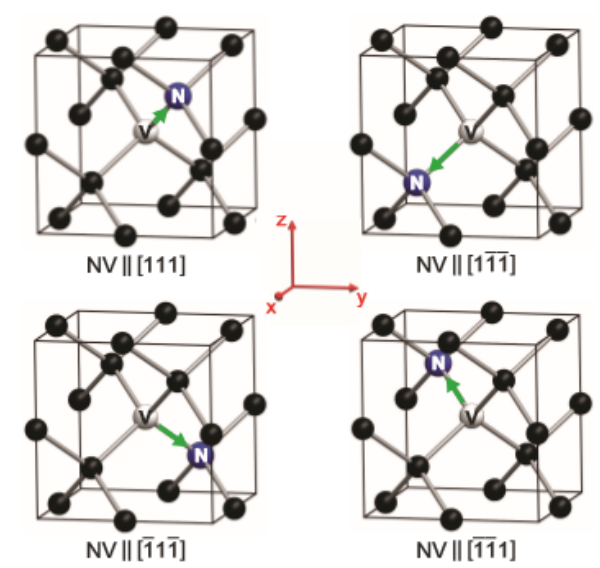
\includegraphics[width=0.5\linewidth]{../figures/NClatt}
 	\caption[Different orientations of the NV centres]{Lattice structure of diamonds with four different orientations of the NV centres. Black points mark carbon atoms, and blue and with the Nitrogen and Void atoms respectively. Taken from \cite{pham_magnetic_nodate}.}
 	\label{fig:nclatt}
 \end{figure}
 
 A simplified quantum structure of the NV$^-$ and NV$^0$ centres can be seen in the figure \ref{fig:nvcentres} where the ground state and excited state are constructed by triplet states with a distance of 1.945 eV in between, here called $^{3}$A$_{2}$ and $^{3}$E respectively. The split-up of the energy level in NV$^-$ centres compared to the NV$^0$ centres cause a secondary decay process using the metastable singlet states $^1$A$_1$ and $^1$E$_1$. The primary decay process is the decay from $^{3}$E to $^{3}$A$_{2}$. For the NV$^-$ centre, this transition has a wavelength of $\lambda_{zpl} = 637\,\mathrm{nm}$ which corresponds to the so-called zero phonon line (ZPL). The ZPL is the peak in the fluorescence spectrum where no phonon excitation is included in the decay. Since the ZPL has another wavelength for the NV$^0$ centres this can be used to differentiate between NV$^-$ and NV$^0$ centres using the fluorescence spectrum \cite{schirhagl_nitrogen-vacancy_2014}.\\

\begin{figure}
	
	\centering
	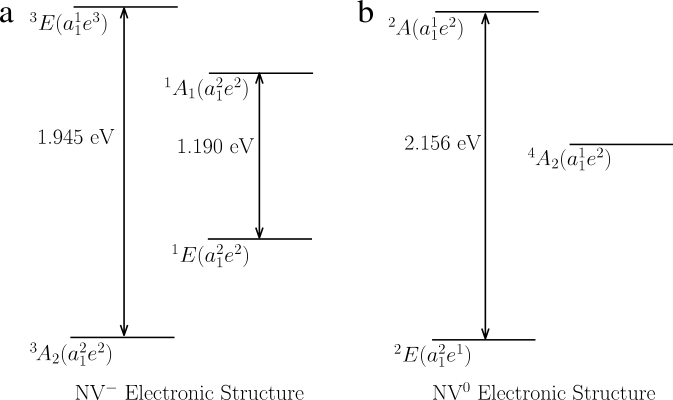
\includegraphics[width=0.5\textwidth]{../figures/nv-centre.png}
	\caption{Electronic structure of (a) NV$^-$ and (b) NV$^0$ centres \cite{doherty}}
	\label{fig:nvcentres}
\end{figure}


The wide properties of NV$^{-}$ centres have made this research gain popularity in wide range of application as temperature sensing \cite{neumann_high-precision_2013}, pressure sensing \cite{doherty_electronic_2014} and even biological applications \cite{mcguinness_quantum_2011}.

%\subsection{Experimental Methods}

\subsection{Optically Detected Magnetic Resonance}
\label{sec:odmr}

Optically detected magnetic resonance (ODMR), is  a  double  resonance  technique  which  combines  optical measurements, in our case the fluorescence of the NV$^{-}$ centres, with  electron  spin  resonance  spectroscopy.  After  the  first triplet-state ODMR experiment in zero magnetic field reported  in 1968 \cite{schmidt_optical_1967}, the  number  of double resonance studies on excited triplet states grew rapidly.  The ground state of a typical organic molecule is a singlet state, and absorption of light leads to excited singlet states \cite{pham_magnetic_nodate}. The pairing of the electron spins is possible only if there is some degree of spin-orbit coupling, If this happens, then the molecule undergoes intersystem crossing (ISC)  and  becomes  a  triplet  state. After an excited molecule crosses into a triplet state, it may remain there a long time because the de-excitation is spin-forbidden \cite{carbonera_optically_2009}.\\

The triplet state of the  $NV^{-}$ in the ground state $\left| g \right\rangle $ at $m=0$ can be created using a wipe of microwaves with a centre of frequency exactly at the energy gap to $\left|g,m=\pm1\right\rangle $, this leads to two important consequence. First that our system is now a triplet state and so the emission at $m=0$ are forbidden now from the excited state $\left\| e,m=0\right\rangle $ and second that this allows to a major percentage of the non radiative emission to be present from $\left\| s\right\rangle $ to the ground state. This detuning in the microwave can be calculated on base the Hamiltonians of each levels and is equal to \cite{schirhagl_nitrogen-vacancy_2014}:\\

\begin{equation}
\omega_{mw}=(E_{\left|g,m=0\right\rangle}-E_{\left|g,m=\pm 1\right\rangle})/ \hbar = 2\pi \cdot 2870MHz 
\end{equation}
Where $\omega_{mw}$ is the frequency of the microwave and E is the energy of each level.//

The spin properties of NV defects can also be used for magnetic field measurements \cite{sage_optical_2013}. In the presence of a static magnetic field, the degeneracy of the NV defect states is lifted by the Zeeman effect. It leads to the appearance of two resonance lines in the electron spin resonance spectrum. The frequency of the splitting resonances is then directly related to the amplitude of the applied magnetic field $B$ along the NV defect axis \cite{lesik_engineering_2015}. The spatial resolution of a single NV scanning probe magnetometer is fundamentally limited by the electron spin wave function, which is in the Angstrom range. For NV centre application in a high sensitivity magnetometer a single NV defect is integrated onto the tip of an atomic force microscope and used as an atomic-sized magnetic field sensor under ambient conditions. \cite{zhou_scanning_2017}.
Using the magnetic field $B$ the magnetic moment $\mu$ will be given by:
\begin{align}
\mu&=\dfrac{\mu_{b}}{\hbar}\cdot g_{s}\cdot s \\
&=\gamma\cdot s
\end{align}
Where $\mu_{b}$ is the Bohr's magnetron $g_{s}\simeq 2$ the g-factor, $s$ the spin and $\gamma$ the gyromagnetic ratio for the free electron \cite{meschede_gerthsen_2015}. At $B\neq 0$ and $\gamma=2\pi*28.951\,\mathrm{\frac{GHz}{T}}$ the energy gaps between the $m_{s}=1$ and $-1$ are given by:
\begin{align}
	\Delta E&=(E_{0}+h \gamma B_{0}*\cos\alpha)-(E_{0}-h \gamma*\cos\alpha) \\	
	&=2*h \gamma B_{0}*\cos\alpha
\end{align}
Where $\alpha $ is the angle between the magnetic field and magnetic moment. The original resonance is split symmetrically into two magnetic ones, which are detuned around the centre frequency $\omega_\text{centre}$:
\begin{equation}
	\omega=\omega_\text{centre}+\gamma B_{0}*\cos\alpha
\end{equation}
This mean that our frequency is not only sensitive to the amplitude of the magnetic field, but also to the orientation between the crystal and the external field. Furthermore, the isolation of the NV centre's intrinsic influences includes stability of this measurement, providing a sensitive tool to detect magnetic fields \cite{meschede_gerthsen_2015}.

